% Created by tikzDevice version 0.12.6 on 2025-04-06 17:01:44
% !TEX encoding = UTF-8 Unicode
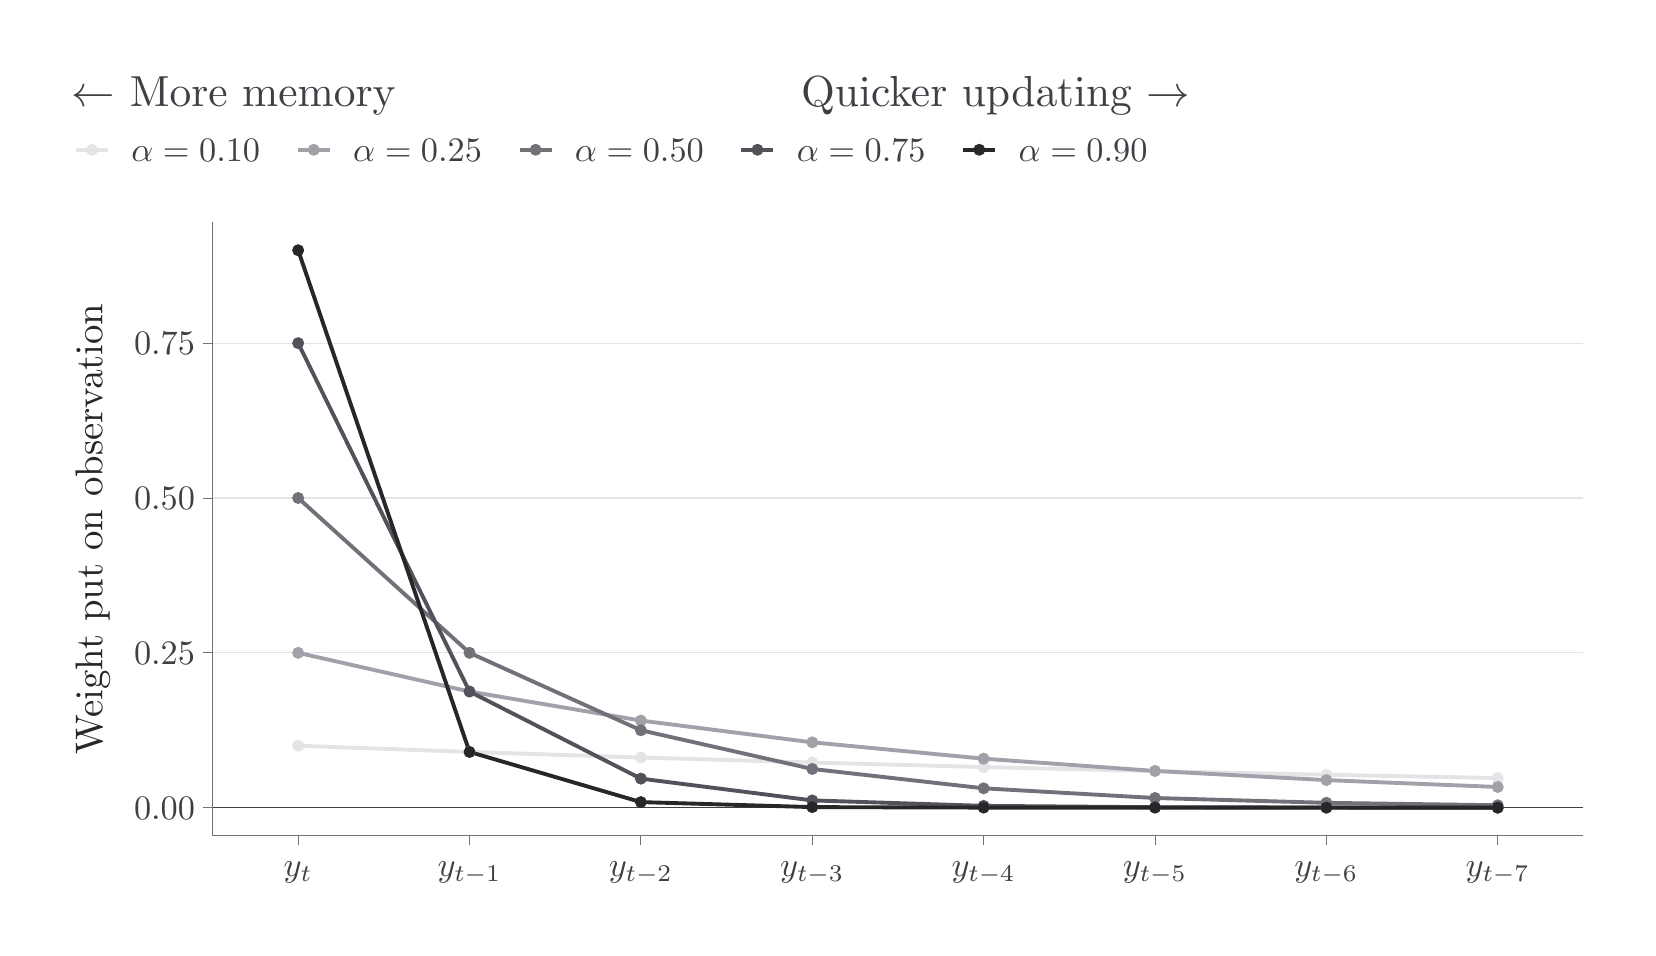
\begin{tikzpicture}[x=1pt,y=1pt]
\definecolor{fillColor}{RGB}{255,255,255}
\path[use as bounding box,fill=fillColor] (0,0) rectangle (578.16,325.21);
\begin{scope}
\path[clip] (  0.00,  0.00) rectangle (578.16,325.21);
\definecolor{drawColor}{RGB}{255,255,255}

\path[draw=drawColor,line width= 0.7pt,line join=round,line cap=round,fill=fillColor] (  0.00,  0.00) rectangle (578.16,325.21);
\end{scope}
\begin{scope}
\path[clip] ( 66.77, 33.29) rectangle (562.16,254.85);
\definecolor{drawColor}{RGB}{255,255,255}
\definecolor{fillColor}{RGB}{255,255,255}

\path[draw=drawColor,line width= 0.7pt,line join=round,line cap=round,fill=fillColor] ( 66.77, 33.29) rectangle (562.16,254.85);
\definecolor{drawColor}{RGB}{228,228,231}

\path[draw=drawColor,line width= 0.4pt,line join=round] ( 66.77, 43.36) --
	(562.16, 43.36);

\path[draw=drawColor,line width= 0.4pt,line join=round] ( 66.77, 99.31) --
	(562.16, 99.31);

\path[draw=drawColor,line width= 0.4pt,line join=round] ( 66.77,155.26) --
	(562.16,155.26);

\path[draw=drawColor,line width= 0.4pt,line join=round] ( 66.77,211.21) --
	(562.16,211.21);
\definecolor{drawColor}{RGB}{63,63,70}

\path[draw=drawColor,line width= 0.6pt,line join=round] ( 66.77, 43.36) -- (562.16, 43.36);
\definecolor{drawColor}{RGB}{228,228,231}

\path[draw=drawColor,line width= 1.4pt,line join=round] ( 97.74, 65.74) --
	(159.66, 63.50) --
	(221.58, 61.49) --
	(283.51, 59.67) --
	(345.43, 58.04) --
	(407.35, 56.57) --
	(469.28, 55.25) --
	(531.20, 54.06);
\definecolor{drawColor}{RGB}{161,161,170}

\path[draw=drawColor,line width= 1.4pt,line join=round] ( 97.74, 99.31) --
	(159.66, 85.32) --
	(221.58, 74.83) --
	(283.51, 66.96) --
	(345.43, 61.06) --
	(407.35, 56.63) --
	(469.28, 53.32) --
	(531.20, 50.83);
\definecolor{drawColor}{RGB}{113,113,122}

\path[draw=drawColor,line width= 1.4pt,line join=round] ( 97.74,155.26) --
	(159.66, 99.31) --
	(221.58, 71.33) --
	(283.51, 57.34) --
	(345.43, 50.35) --
	(407.35, 46.85) --
	(469.28, 45.11) --
	(531.20, 44.23);
\definecolor{drawColor}{RGB}{82,82,91}

\path[draw=drawColor,line width= 1.4pt,line join=round] ( 97.74,211.21) --
	(159.66, 85.32) --
	(221.58, 53.85) --
	(283.51, 45.98) --
	(345.43, 44.01) --
	(407.35, 43.52) --
	(469.28, 43.40) --
	(531.20, 43.37);
\definecolor{drawColor}{RGB}{39,39,42}

\path[draw=drawColor,line width= 1.4pt,line join=round] ( 97.74,244.78) --
	(159.66, 63.50) --
	(221.58, 45.37) --
	(283.51, 43.56) --
	(345.43, 43.38) --
	(407.35, 43.36) --
	(469.28, 43.36) --
	(531.20, 43.36);
\definecolor{drawColor}{RGB}{228,228,231}
\definecolor{fillColor}{RGB}{228,228,231}

\path[draw=drawColor,line width= 0.4pt,line join=round,line cap=round,fill=fillColor] ( 97.74, 65.74) circle (  1.96);

\path[draw=drawColor,line width= 0.4pt,line join=round,line cap=round,fill=fillColor] (159.66, 63.50) circle (  1.96);

\path[draw=drawColor,line width= 0.4pt,line join=round,line cap=round,fill=fillColor] (221.58, 61.49) circle (  1.96);

\path[draw=drawColor,line width= 0.4pt,line join=round,line cap=round,fill=fillColor] (283.51, 59.67) circle (  1.96);

\path[draw=drawColor,line width= 0.4pt,line join=round,line cap=round,fill=fillColor] (345.43, 58.04) circle (  1.96);

\path[draw=drawColor,line width= 0.4pt,line join=round,line cap=round,fill=fillColor] (407.35, 56.57) circle (  1.96);

\path[draw=drawColor,line width= 0.4pt,line join=round,line cap=round,fill=fillColor] (469.28, 55.25) circle (  1.96);

\path[draw=drawColor,line width= 0.4pt,line join=round,line cap=round,fill=fillColor] (531.20, 54.06) circle (  1.96);
\definecolor{drawColor}{RGB}{161,161,170}
\definecolor{fillColor}{RGB}{161,161,170}

\path[draw=drawColor,line width= 0.4pt,line join=round,line cap=round,fill=fillColor] ( 97.74, 99.31) circle (  1.96);

\path[draw=drawColor,line width= 0.4pt,line join=round,line cap=round,fill=fillColor] (159.66, 85.32) circle (  1.96);

\path[draw=drawColor,line width= 0.4pt,line join=round,line cap=round,fill=fillColor] (221.58, 74.83) circle (  1.96);

\path[draw=drawColor,line width= 0.4pt,line join=round,line cap=round,fill=fillColor] (283.51, 66.96) circle (  1.96);

\path[draw=drawColor,line width= 0.4pt,line join=round,line cap=round,fill=fillColor] (345.43, 61.06) circle (  1.96);

\path[draw=drawColor,line width= 0.4pt,line join=round,line cap=round,fill=fillColor] (407.35, 56.63) circle (  1.96);

\path[draw=drawColor,line width= 0.4pt,line join=round,line cap=round,fill=fillColor] (469.28, 53.32) circle (  1.96);

\path[draw=drawColor,line width= 0.4pt,line join=round,line cap=round,fill=fillColor] (531.20, 50.83) circle (  1.96);
\definecolor{drawColor}{RGB}{113,113,122}
\definecolor{fillColor}{RGB}{113,113,122}

\path[draw=drawColor,line width= 0.4pt,line join=round,line cap=round,fill=fillColor] ( 97.74,155.26) circle (  1.96);

\path[draw=drawColor,line width= 0.4pt,line join=round,line cap=round,fill=fillColor] (159.66, 99.31) circle (  1.96);

\path[draw=drawColor,line width= 0.4pt,line join=round,line cap=round,fill=fillColor] (221.58, 71.33) circle (  1.96);

\path[draw=drawColor,line width= 0.4pt,line join=round,line cap=round,fill=fillColor] (283.51, 57.34) circle (  1.96);

\path[draw=drawColor,line width= 0.4pt,line join=round,line cap=round,fill=fillColor] (345.43, 50.35) circle (  1.96);

\path[draw=drawColor,line width= 0.4pt,line join=round,line cap=round,fill=fillColor] (407.35, 46.85) circle (  1.96);

\path[draw=drawColor,line width= 0.4pt,line join=round,line cap=round,fill=fillColor] (469.28, 45.11) circle (  1.96);

\path[draw=drawColor,line width= 0.4pt,line join=round,line cap=round,fill=fillColor] (531.20, 44.23) circle (  1.96);
\definecolor{drawColor}{RGB}{82,82,91}
\definecolor{fillColor}{RGB}{82,82,91}

\path[draw=drawColor,line width= 0.4pt,line join=round,line cap=round,fill=fillColor] ( 97.74,211.21) circle (  1.96);

\path[draw=drawColor,line width= 0.4pt,line join=round,line cap=round,fill=fillColor] (159.66, 85.32) circle (  1.96);

\path[draw=drawColor,line width= 0.4pt,line join=round,line cap=round,fill=fillColor] (221.58, 53.85) circle (  1.96);

\path[draw=drawColor,line width= 0.4pt,line join=round,line cap=round,fill=fillColor] (283.51, 45.98) circle (  1.96);

\path[draw=drawColor,line width= 0.4pt,line join=round,line cap=round,fill=fillColor] (345.43, 44.01) circle (  1.96);

\path[draw=drawColor,line width= 0.4pt,line join=round,line cap=round,fill=fillColor] (407.35, 43.52) circle (  1.96);

\path[draw=drawColor,line width= 0.4pt,line join=round,line cap=round,fill=fillColor] (469.28, 43.40) circle (  1.96);

\path[draw=drawColor,line width= 0.4pt,line join=round,line cap=round,fill=fillColor] (531.20, 43.37) circle (  1.96);
\definecolor{drawColor}{RGB}{39,39,42}
\definecolor{fillColor}{RGB}{39,39,42}

\path[draw=drawColor,line width= 0.4pt,line join=round,line cap=round,fill=fillColor] ( 97.74,244.78) circle (  1.96);

\path[draw=drawColor,line width= 0.4pt,line join=round,line cap=round,fill=fillColor] (159.66, 63.50) circle (  1.96);

\path[draw=drawColor,line width= 0.4pt,line join=round,line cap=round,fill=fillColor] (221.58, 45.37) circle (  1.96);

\path[draw=drawColor,line width= 0.4pt,line join=round,line cap=round,fill=fillColor] (283.51, 43.56) circle (  1.96);

\path[draw=drawColor,line width= 0.4pt,line join=round,line cap=round,fill=fillColor] (345.43, 43.38) circle (  1.96);

\path[draw=drawColor,line width= 0.4pt,line join=round,line cap=round,fill=fillColor] (407.35, 43.36) circle (  1.96);

\path[draw=drawColor,line width= 0.4pt,line join=round,line cap=round,fill=fillColor] (469.28, 43.36) circle (  1.96);

\path[draw=drawColor,line width= 0.4pt,line join=round,line cap=round,fill=fillColor] (531.20, 43.36) circle (  1.96);
\end{scope}
\begin{scope}
\path[clip] (  0.00,  0.00) rectangle (578.16,325.21);
\definecolor{drawColor}{RGB}{113,113,122}

\path[draw=drawColor,line width= 0.3pt,line join=round] ( 66.77, 33.29) --
	( 66.77,254.85);
\end{scope}
\begin{scope}
\path[clip] (  0.00,  0.00) rectangle (578.16,325.21);
\definecolor{drawColor}{RGB}{63,63,70}

\node[text=drawColor,anchor=base east,inner sep=0pt, outer sep=0pt, scale=  1.24] at ( 60.47, 39.07) {0.00};

\node[text=drawColor,anchor=base east,inner sep=0pt, outer sep=0pt, scale=  1.24] at ( 60.47, 95.02) {0.25};

\node[text=drawColor,anchor=base east,inner sep=0pt, outer sep=0pt, scale=  1.24] at ( 60.47,150.98) {0.50};

\node[text=drawColor,anchor=base east,inner sep=0pt, outer sep=0pt, scale=  1.24] at ( 60.47,206.93) {0.75};
\end{scope}
\begin{scope}
\path[clip] (  0.00,  0.00) rectangle (578.16,325.21);
\definecolor{drawColor}{RGB}{113,113,122}

\path[draw=drawColor,line width= 0.3pt,line join=round] ( 63.27, 43.36) --
	( 66.77, 43.36);

\path[draw=drawColor,line width= 0.3pt,line join=round] ( 63.27, 99.31) --
	( 66.77, 99.31);

\path[draw=drawColor,line width= 0.3pt,line join=round] ( 63.27,155.26) --
	( 66.77,155.26);

\path[draw=drawColor,line width= 0.3pt,line join=round] ( 63.27,211.21) --
	( 66.77,211.21);
\end{scope}
\begin{scope}
\path[clip] (  0.00,  0.00) rectangle (578.16,325.21);
\definecolor{drawColor}{RGB}{113,113,122}

\path[draw=drawColor,line width= 0.3pt,line join=round] ( 66.77, 33.29) --
	(562.16, 33.29);
\end{scope}
\begin{scope}
\path[clip] (  0.00,  0.00) rectangle (578.16,325.21);
\definecolor{drawColor}{RGB}{113,113,122}

\path[draw=drawColor,line width= 0.3pt,line join=round] ( 97.74, 29.79) --
	( 97.74, 33.29);

\path[draw=drawColor,line width= 0.3pt,line join=round] (159.66, 29.79) --
	(159.66, 33.29);

\path[draw=drawColor,line width= 0.3pt,line join=round] (221.58, 29.79) --
	(221.58, 33.29);

\path[draw=drawColor,line width= 0.3pt,line join=round] (283.51, 29.79) --
	(283.51, 33.29);

\path[draw=drawColor,line width= 0.3pt,line join=round] (345.43, 29.79) --
	(345.43, 33.29);

\path[draw=drawColor,line width= 0.3pt,line join=round] (407.35, 29.79) --
	(407.35, 33.29);

\path[draw=drawColor,line width= 0.3pt,line join=round] (469.28, 29.79) --
	(469.28, 33.29);

\path[draw=drawColor,line width= 0.3pt,line join=round] (531.20, 29.79) --
	(531.20, 33.29);
\end{scope}
\begin{scope}
\path[clip] (  0.00,  0.00) rectangle (578.16,325.21);
\definecolor{drawColor}{RGB}{63,63,70}

\node[text=drawColor,anchor=base,inner sep=0pt, outer sep=0pt, scale=  1.24] at ( 97.74, 18.42) {$y_t$};

\node[text=drawColor,anchor=base,inner sep=0pt, outer sep=0pt, scale=  1.24] at (159.66, 18.42) {$y_{t-1}$};

\node[text=drawColor,anchor=base,inner sep=0pt, outer sep=0pt, scale=  1.24] at (221.58, 18.42) {$y_{t-2}$};

\node[text=drawColor,anchor=base,inner sep=0pt, outer sep=0pt, scale=  1.24] at (283.51, 18.42) {$y_{t-3}$};

\node[text=drawColor,anchor=base,inner sep=0pt, outer sep=0pt, scale=  1.24] at (345.43, 18.42) {$y_{t-4}$};

\node[text=drawColor,anchor=base,inner sep=0pt, outer sep=0pt, scale=  1.24] at (407.35, 18.42) {$y_{t-5}$};

\node[text=drawColor,anchor=base,inner sep=0pt, outer sep=0pt, scale=  1.24] at (469.28, 18.42) {$y_{t-6}$};

\node[text=drawColor,anchor=base,inner sep=0pt, outer sep=0pt, scale=  1.24] at (531.20, 18.42) {$y_{t-7}$};
\end{scope}
\begin{scope}
\path[clip] (  0.00,  0.00) rectangle (578.16,325.21);
\definecolor{drawColor}{RGB}{39,39,42}

\node[text=drawColor,rotate= 90.00,anchor=base,inner sep=0pt, outer sep=0pt, scale=  1.40] at ( 27.00,144.07) {Weight put on observation};
\end{scope}
\begin{scope}
\path[clip] (  0.00,  0.00) rectangle (578.16,325.21);
\definecolor{drawColor}{RGB}{255,255,255}
\definecolor{fillColor}{RGB}{255,255,255}

\path[draw=drawColor,line width= 0.7pt,line join=round,line cap=round,fill=fillColor] ( 16.00,268.85) rectangle (421.16,309.21);
\end{scope}
\begin{scope}
\path[clip] (  0.00,  0.00) rectangle (578.16,325.21);
\definecolor{drawColor}{RGB}{63,63,70}

\node[text=drawColor,anchor=base west,inner sep=0pt, outer sep=0pt, scale=  1.57] at ( 16.00,296.84) {$\leftarrow$ More memory \qquad \qquad \qquad \qquad \quad Quicker updating $\rightarrow$};
\end{scope}
\begin{scope}
\path[clip] (  0.00,  0.00) rectangle (578.16,325.21);
\definecolor{drawColor}{RGB}{255,255,255}
\definecolor{fillColor}{RGB}{255,255,255}

\path[draw=drawColor,line width= 0.7pt,line join=round,line cap=round,fill=fillColor] ( 16.00,273.85) rectangle ( 30.45,288.31);
\end{scope}
\begin{scope}
\path[clip] (  0.00,  0.00) rectangle (578.16,325.21);
\definecolor{drawColor}{RGB}{228,228,231}

\path[draw=drawColor,line width= 1.4pt,line join=round] ( 17.45,281.08) -- ( 29.01,281.08);
\end{scope}
\begin{scope}
\path[clip] (  0.00,  0.00) rectangle (578.16,325.21);
\definecolor{drawColor}{RGB}{228,228,231}
\definecolor{fillColor}{RGB}{228,228,231}

\path[draw=drawColor,line width= 0.4pt,line join=round,line cap=round,fill=fillColor] ( 23.23,281.08) circle (  1.96);
\end{scope}
\begin{scope}
\path[clip] (  0.00,  0.00) rectangle (578.16,325.21);
\definecolor{drawColor}{RGB}{255,255,255}
\definecolor{fillColor}{RGB}{255,255,255}

\path[draw=drawColor,line width= 0.7pt,line join=round,line cap=round,fill=fillColor] ( 96.16,273.85) rectangle (110.61,288.31);
\end{scope}
\begin{scope}
\path[clip] (  0.00,  0.00) rectangle (578.16,325.21);
\definecolor{drawColor}{RGB}{161,161,170}

\path[draw=drawColor,line width= 1.4pt,line join=round] ( 97.61,281.08) -- (109.17,281.08);
\end{scope}
\begin{scope}
\path[clip] (  0.00,  0.00) rectangle (578.16,325.21);
\definecolor{drawColor}{RGB}{161,161,170}
\definecolor{fillColor}{RGB}{161,161,170}

\path[draw=drawColor,line width= 0.4pt,line join=round,line cap=round,fill=fillColor] (103.39,281.08) circle (  1.96);
\end{scope}
\begin{scope}
\path[clip] (  0.00,  0.00) rectangle (578.16,325.21);
\definecolor{drawColor}{RGB}{255,255,255}
\definecolor{fillColor}{RGB}{255,255,255}

\path[draw=drawColor,line width= 0.7pt,line join=round,line cap=round,fill=fillColor] (176.32,273.85) rectangle (190.77,288.31);
\end{scope}
\begin{scope}
\path[clip] (  0.00,  0.00) rectangle (578.16,325.21);
\definecolor{drawColor}{RGB}{113,113,122}

\path[draw=drawColor,line width= 1.4pt,line join=round] (177.77,281.08) -- (189.33,281.08);
\end{scope}
\begin{scope}
\path[clip] (  0.00,  0.00) rectangle (578.16,325.21);
\definecolor{drawColor}{RGB}{113,113,122}
\definecolor{fillColor}{RGB}{113,113,122}

\path[draw=drawColor,line width= 0.4pt,line join=round,line cap=round,fill=fillColor] (183.55,281.08) circle (  1.96);
\end{scope}
\begin{scope}
\path[clip] (  0.00,  0.00) rectangle (578.16,325.21);
\definecolor{drawColor}{RGB}{255,255,255}
\definecolor{fillColor}{RGB}{255,255,255}

\path[draw=drawColor,line width= 0.7pt,line join=round,line cap=round,fill=fillColor] (256.48,273.85) rectangle (270.93,288.31);
\end{scope}
\begin{scope}
\path[clip] (  0.00,  0.00) rectangle (578.16,325.21);
\definecolor{drawColor}{RGB}{82,82,91}

\path[draw=drawColor,line width= 1.4pt,line join=round] (257.93,281.08) -- (269.49,281.08);
\end{scope}
\begin{scope}
\path[clip] (  0.00,  0.00) rectangle (578.16,325.21);
\definecolor{drawColor}{RGB}{82,82,91}
\definecolor{fillColor}{RGB}{82,82,91}

\path[draw=drawColor,line width= 0.4pt,line join=round,line cap=round,fill=fillColor] (263.71,281.08) circle (  1.96);
\end{scope}
\begin{scope}
\path[clip] (  0.00,  0.00) rectangle (578.16,325.21);
\definecolor{drawColor}{RGB}{255,255,255}
\definecolor{fillColor}{RGB}{255,255,255}

\path[draw=drawColor,line width= 0.7pt,line join=round,line cap=round,fill=fillColor] (336.64,273.85) rectangle (351.09,288.31);
\end{scope}
\begin{scope}
\path[clip] (  0.00,  0.00) rectangle (578.16,325.21);
\definecolor{drawColor}{RGB}{39,39,42}

\path[draw=drawColor,line width= 1.4pt,line join=round] (338.09,281.08) -- (349.65,281.08);
\end{scope}
\begin{scope}
\path[clip] (  0.00,  0.00) rectangle (578.16,325.21);
\definecolor{drawColor}{RGB}{39,39,42}
\definecolor{fillColor}{RGB}{39,39,42}

\path[draw=drawColor,line width= 0.4pt,line join=round,line cap=round,fill=fillColor] (343.87,281.08) circle (  1.96);
\end{scope}
\begin{scope}
\path[clip] (  0.00,  0.00) rectangle (578.16,325.21);
\definecolor{drawColor}{RGB}{63,63,70}

\node[text=drawColor,anchor=base west,inner sep=0pt, outer sep=0pt, scale=  1.24] at ( 37.45,276.80) {$\alpha = 0.10$};
\end{scope}
\begin{scope}
\path[clip] (  0.00,  0.00) rectangle (578.16,325.21);
\definecolor{drawColor}{RGB}{63,63,70}

\node[text=drawColor,anchor=base west,inner sep=0pt, outer sep=0pt, scale=  1.24] at (117.61,276.80) {$\alpha = 0.25$};
\end{scope}
\begin{scope}
\path[clip] (  0.00,  0.00) rectangle (578.16,325.21);
\definecolor{drawColor}{RGB}{63,63,70}

\node[text=drawColor,anchor=base west,inner sep=0pt, outer sep=0pt, scale=  1.24] at (197.77,276.80) {$\alpha = 0.50$};
\end{scope}
\begin{scope}
\path[clip] (  0.00,  0.00) rectangle (578.16,325.21);
\definecolor{drawColor}{RGB}{63,63,70}

\node[text=drawColor,anchor=base west,inner sep=0pt, outer sep=0pt, scale=  1.24] at (277.93,276.80) {$\alpha = 0.75$};
\end{scope}
\begin{scope}
\path[clip] (  0.00,  0.00) rectangle (578.16,325.21);
\definecolor{drawColor}{RGB}{63,63,70}

\node[text=drawColor,anchor=base west,inner sep=0pt, outer sep=0pt, scale=  1.24] at (358.09,276.80) {$\alpha = 0.90$};
\end{scope}
\end{tikzpicture}
